% Options for packages loaded elsewhere
\PassOptionsToPackage{unicode}{hyperref}
\PassOptionsToPackage{hyphens}{url}
%
\documentclass[
]{book}
\usepackage{amsmath,amssymb}
\usepackage{iftex}
\ifPDFTeX
  \usepackage[T1]{fontenc}
  \usepackage[utf8]{inputenc}
  \usepackage{textcomp} % provide euro and other symbols
\else % if luatex or xetex
  \usepackage{unicode-math} % this also loads fontspec
  \defaultfontfeatures{Scale=MatchLowercase}
  \defaultfontfeatures[\rmfamily]{Ligatures=TeX,Scale=1}
\fi
\usepackage{lmodern}
\ifPDFTeX\else
  % xetex/luatex font selection
\fi
% Use upquote if available, for straight quotes in verbatim environments
\IfFileExists{upquote.sty}{\usepackage{upquote}}{}
\IfFileExists{microtype.sty}{% use microtype if available
  \usepackage[]{microtype}
  \UseMicrotypeSet[protrusion]{basicmath} % disable protrusion for tt fonts
}{}
\makeatletter
\@ifundefined{KOMAClassName}{% if non-KOMA class
  \IfFileExists{parskip.sty}{%
    \usepackage{parskip}
  }{% else
    \setlength{\parindent}{0pt}
    \setlength{\parskip}{6pt plus 2pt minus 1pt}}
}{% if KOMA class
  \KOMAoptions{parskip=half}}
\makeatother
\usepackage{xcolor}
\usepackage{color}
\usepackage{fancyvrb}
\newcommand{\VerbBar}{|}
\newcommand{\VERB}{\Verb[commandchars=\\\{\}]}
\DefineVerbatimEnvironment{Highlighting}{Verbatim}{commandchars=\\\{\}}
% Add ',fontsize=\small' for more characters per line
\usepackage{framed}
\definecolor{shadecolor}{RGB}{248,248,248}
\newenvironment{Shaded}{\begin{snugshade}}{\end{snugshade}}
\newcommand{\AlertTok}[1]{\textcolor[rgb]{0.94,0.16,0.16}{#1}}
\newcommand{\AnnotationTok}[1]{\textcolor[rgb]{0.56,0.35,0.01}{\textbf{\textit{#1}}}}
\newcommand{\AttributeTok}[1]{\textcolor[rgb]{0.13,0.29,0.53}{#1}}
\newcommand{\BaseNTok}[1]{\textcolor[rgb]{0.00,0.00,0.81}{#1}}
\newcommand{\BuiltInTok}[1]{#1}
\newcommand{\CharTok}[1]{\textcolor[rgb]{0.31,0.60,0.02}{#1}}
\newcommand{\CommentTok}[1]{\textcolor[rgb]{0.56,0.35,0.01}{\textit{#1}}}
\newcommand{\CommentVarTok}[1]{\textcolor[rgb]{0.56,0.35,0.01}{\textbf{\textit{#1}}}}
\newcommand{\ConstantTok}[1]{\textcolor[rgb]{0.56,0.35,0.01}{#1}}
\newcommand{\ControlFlowTok}[1]{\textcolor[rgb]{0.13,0.29,0.53}{\textbf{#1}}}
\newcommand{\DataTypeTok}[1]{\textcolor[rgb]{0.13,0.29,0.53}{#1}}
\newcommand{\DecValTok}[1]{\textcolor[rgb]{0.00,0.00,0.81}{#1}}
\newcommand{\DocumentationTok}[1]{\textcolor[rgb]{0.56,0.35,0.01}{\textbf{\textit{#1}}}}
\newcommand{\ErrorTok}[1]{\textcolor[rgb]{0.64,0.00,0.00}{\textbf{#1}}}
\newcommand{\ExtensionTok}[1]{#1}
\newcommand{\FloatTok}[1]{\textcolor[rgb]{0.00,0.00,0.81}{#1}}
\newcommand{\FunctionTok}[1]{\textcolor[rgb]{0.13,0.29,0.53}{\textbf{#1}}}
\newcommand{\ImportTok}[1]{#1}
\newcommand{\InformationTok}[1]{\textcolor[rgb]{0.56,0.35,0.01}{\textbf{\textit{#1}}}}
\newcommand{\KeywordTok}[1]{\textcolor[rgb]{0.13,0.29,0.53}{\textbf{#1}}}
\newcommand{\NormalTok}[1]{#1}
\newcommand{\OperatorTok}[1]{\textcolor[rgb]{0.81,0.36,0.00}{\textbf{#1}}}
\newcommand{\OtherTok}[1]{\textcolor[rgb]{0.56,0.35,0.01}{#1}}
\newcommand{\PreprocessorTok}[1]{\textcolor[rgb]{0.56,0.35,0.01}{\textit{#1}}}
\newcommand{\RegionMarkerTok}[1]{#1}
\newcommand{\SpecialCharTok}[1]{\textcolor[rgb]{0.81,0.36,0.00}{\textbf{#1}}}
\newcommand{\SpecialStringTok}[1]{\textcolor[rgb]{0.31,0.60,0.02}{#1}}
\newcommand{\StringTok}[1]{\textcolor[rgb]{0.31,0.60,0.02}{#1}}
\newcommand{\VariableTok}[1]{\textcolor[rgb]{0.00,0.00,0.00}{#1}}
\newcommand{\VerbatimStringTok}[1]{\textcolor[rgb]{0.31,0.60,0.02}{#1}}
\newcommand{\WarningTok}[1]{\textcolor[rgb]{0.56,0.35,0.01}{\textbf{\textit{#1}}}}
\usepackage{longtable,booktabs,array}
\usepackage{calc} % for calculating minipage widths
% Correct order of tables after \paragraph or \subparagraph
\usepackage{etoolbox}
\makeatletter
\patchcmd\longtable{\par}{\if@noskipsec\mbox{}\fi\par}{}{}
\makeatother
% Allow footnotes in longtable head/foot
\IfFileExists{footnotehyper.sty}{\usepackage{footnotehyper}}{\usepackage{footnote}}
\makesavenoteenv{longtable}
\usepackage{graphicx}
\makeatletter
\def\maxwidth{\ifdim\Gin@nat@width>\linewidth\linewidth\else\Gin@nat@width\fi}
\def\maxheight{\ifdim\Gin@nat@height>\textheight\textheight\else\Gin@nat@height\fi}
\makeatother
% Scale images if necessary, so that they will not overflow the page
% margins by default, and it is still possible to overwrite the defaults
% using explicit options in \includegraphics[width, height, ...]{}
\setkeys{Gin}{width=\maxwidth,height=\maxheight,keepaspectratio}
% Set default figure placement to htbp
\makeatletter
\def\fps@figure{htbp}
\makeatother
\setlength{\emergencystretch}{3em} % prevent overfull lines
\providecommand{\tightlist}{%
  \setlength{\itemsep}{0pt}\setlength{\parskip}{0pt}}
\setcounter{secnumdepth}{5}
\usepackage{booktabs}
\ifLuaTeX
  \usepackage{selnolig}  % disable illegal ligatures
\fi
\usepackage[]{natbib}
\bibliographystyle{plainnat}
\IfFileExists{bookmark.sty}{\usepackage{bookmark}}{\usepackage{hyperref}}
\IfFileExists{xurl.sty}{\usepackage{xurl}}{} % add URL line breaks if available
\urlstyle{same}
\hypersetup{
  pdftitle={BMP Dashboard Manual},
  pdfauthor={Ané Cloete},
  hidelinks,
  pdfcreator={LaTeX via pandoc}}

\title{BMP Dashboard Manual}
\author{Ané Cloete}
\date{2023-10-05}

\usepackage{amsthm}
\newtheorem{theorem}{Theorem}[chapter]
\newtheorem{lemma}{Lemma}[chapter]
\newtheorem{corollary}{Corollary}[chapter]
\newtheorem{proposition}{Proposition}[chapter]
\newtheorem{conjecture}{Conjecture}[chapter]
\theoremstyle{definition}
\newtheorem{definition}{Definition}[chapter]
\theoremstyle{definition}
\newtheorem{example}{Example}[chapter]
\theoremstyle{definition}
\newtheorem{exercise}{Exercise}[chapter]
\theoremstyle{definition}
\newtheorem{hypothesis}{Hypothesis}[chapter]
\theoremstyle{remark}
\newtheorem*{remark}{Remark}
\newtheorem*{solution}{Solution}
\begin{document}
\maketitle

{
\setcounter{tocdepth}{1}
\tableofcontents
}
\hypertarget{hi}{%
\chapter{Hi :)}\label{hi}}

Everything you need to know to takeover the maintaining and building of the BMP dashboard is in this bookdown. The first chapter will outline the R project folder structure and contents and then in Chapter two I'll talk about how to get the biodiversity data form OneDrive and prepare the data for the dashboard. The remaining chapters will delve into the code itself.

Before starting, here is a short list of handy resources:

\begin{itemize}
\tightlist
\item
  \href{https://bookdown.org/yih_huynh/Guide-to-R-Book/}{R}
\item
  \href{https://mastering-shiny.org/}{Shiny}
\item
  \href{https://happygitwithr.com/existing-github-last}{Github}
\item
  \href{https://bookdown.org/yihui/bookdown/get-started.html}{Bookdown} (if you want to know how to make something like this).
\end{itemize}

These are big and comprehensive resources that will aid you along the way. But remember google and \href{https://stackoverflow.com/}{stackoverflow} are your best friends! And ChatGPT might become your closest and most frustrating colleague.

\hypertarget{owners}{%
\section{Owners}\label{owners}}

\begin{itemize}
\tightlist
\item
  \href{https://www.linkedin.com/in/an\%C3\%A9-c-95629ab5/}{Ané Cloete} (2023)
\end{itemize}

If you are the new dashboard manager, add your name as well! All you need to do is open the bookdown project and navigate to the ``index.Rmd'' file and scroll down till you see this section. In the next chapter you'll see where this folder is located.

Remember the dashboard is work in progress, so feel free to change and modify it as you like and most importantly have fun with it! Let's begin!

\hypertarget{files-within-folders-and-folders-within-files-and-more-files}{%
\chapter{Files within folders and folders within files and more files}\label{files-within-folders-and-folders-within-files-and-more-files}}

Let's go over all the files and folders you've now gotten access to starting with the OneDrive Folder.

\hypertarget{biodiversity-kpi-mapping-master}{%
\section{Biodiversity KPI mapping Master}\label{biodiversity-kpi-mapping-master}}

This is, as it's name suggests, the master folder! And all the NB things are stored here, this is what you should see (unless more folders have been added since the creation of this bookdown 😅). But don't fret, you probably know about these folders already and the most important folders for the dashboard are: \textbf{Team\_Data}, \textbf{Survey\_Photos} and \textbf{Biodiversity Survey Master}.

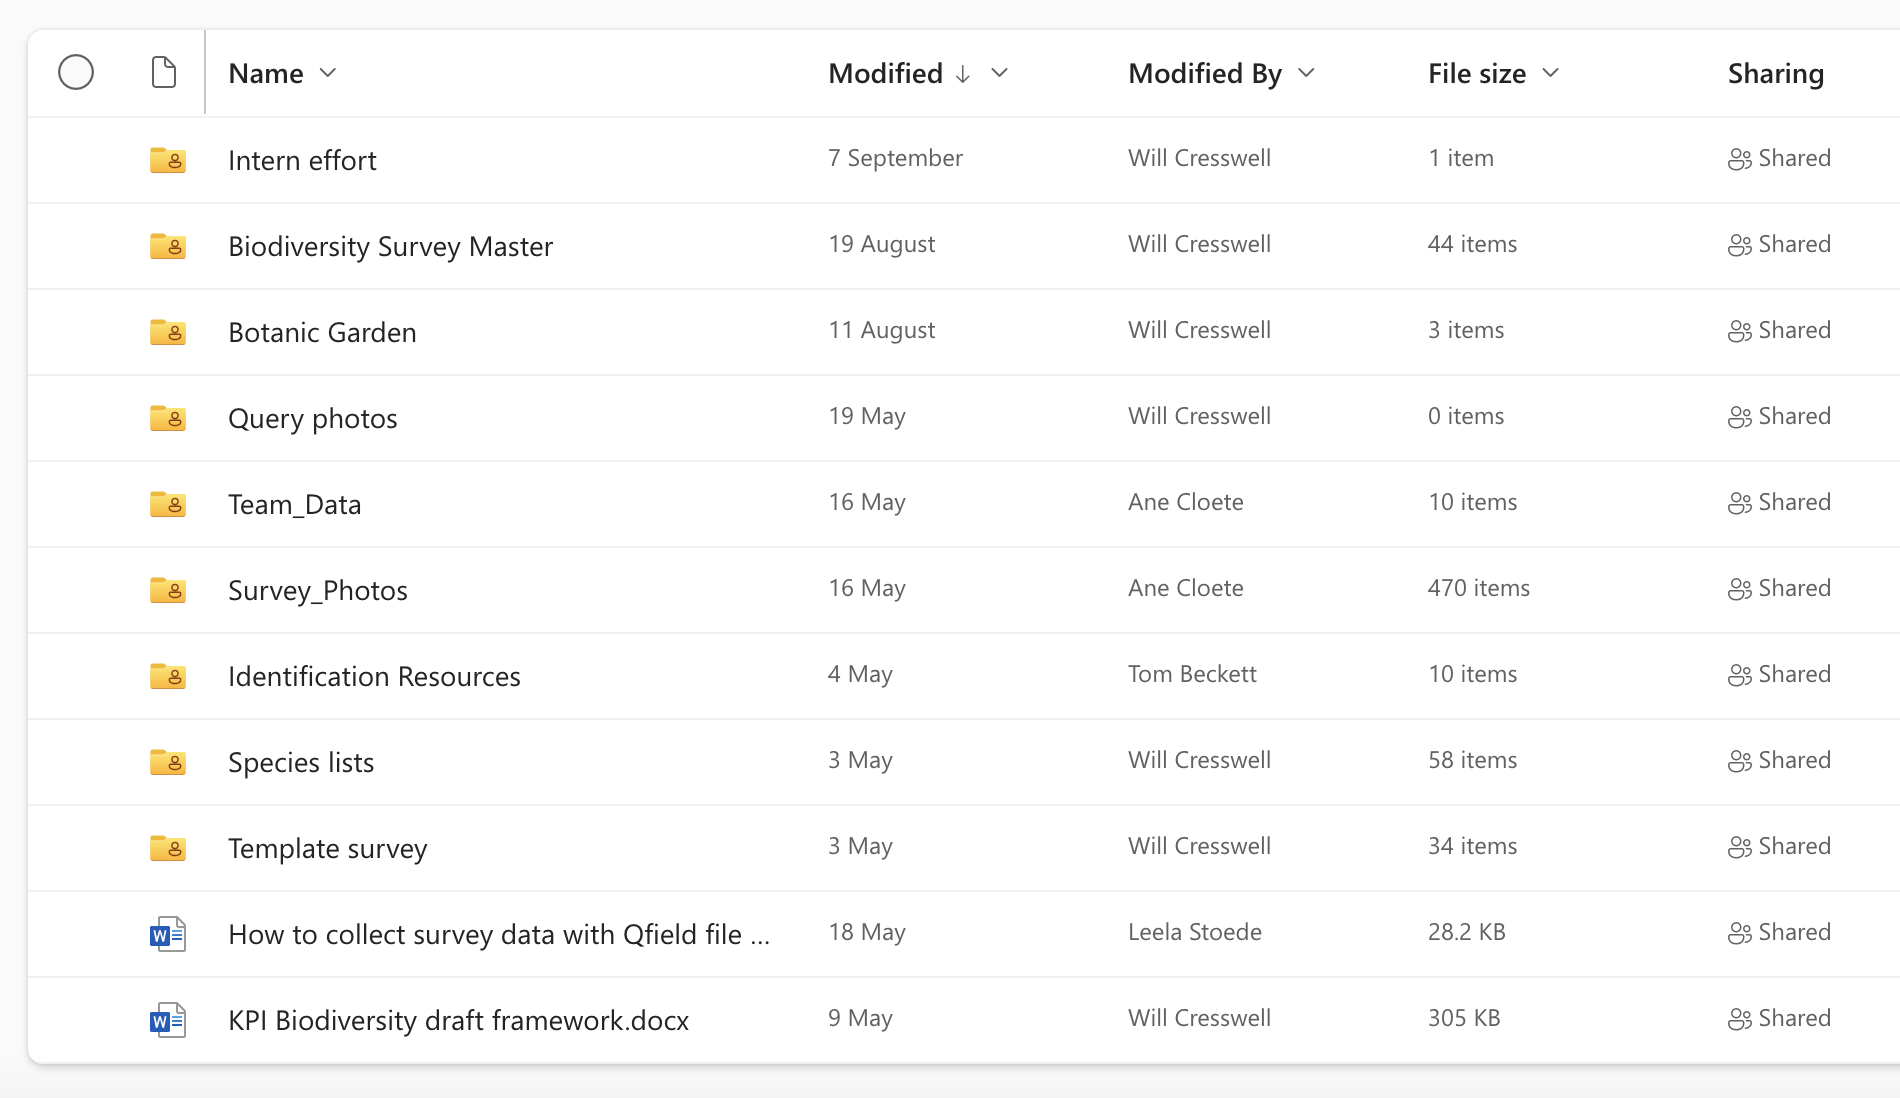
\includegraphics{images/KPI_contents.png}

\hypertarget{biodiversity-survey-master}{%
\subsection{Biodiversity Survey Master}\label{biodiversity-survey-master}}

Here is where all the students upload their biodiversity data. Each student has their own folder labelled with their names and within each folder all the geopackages for each taxa they have collected data on is stored (plus another folder containing backups), e.g.~

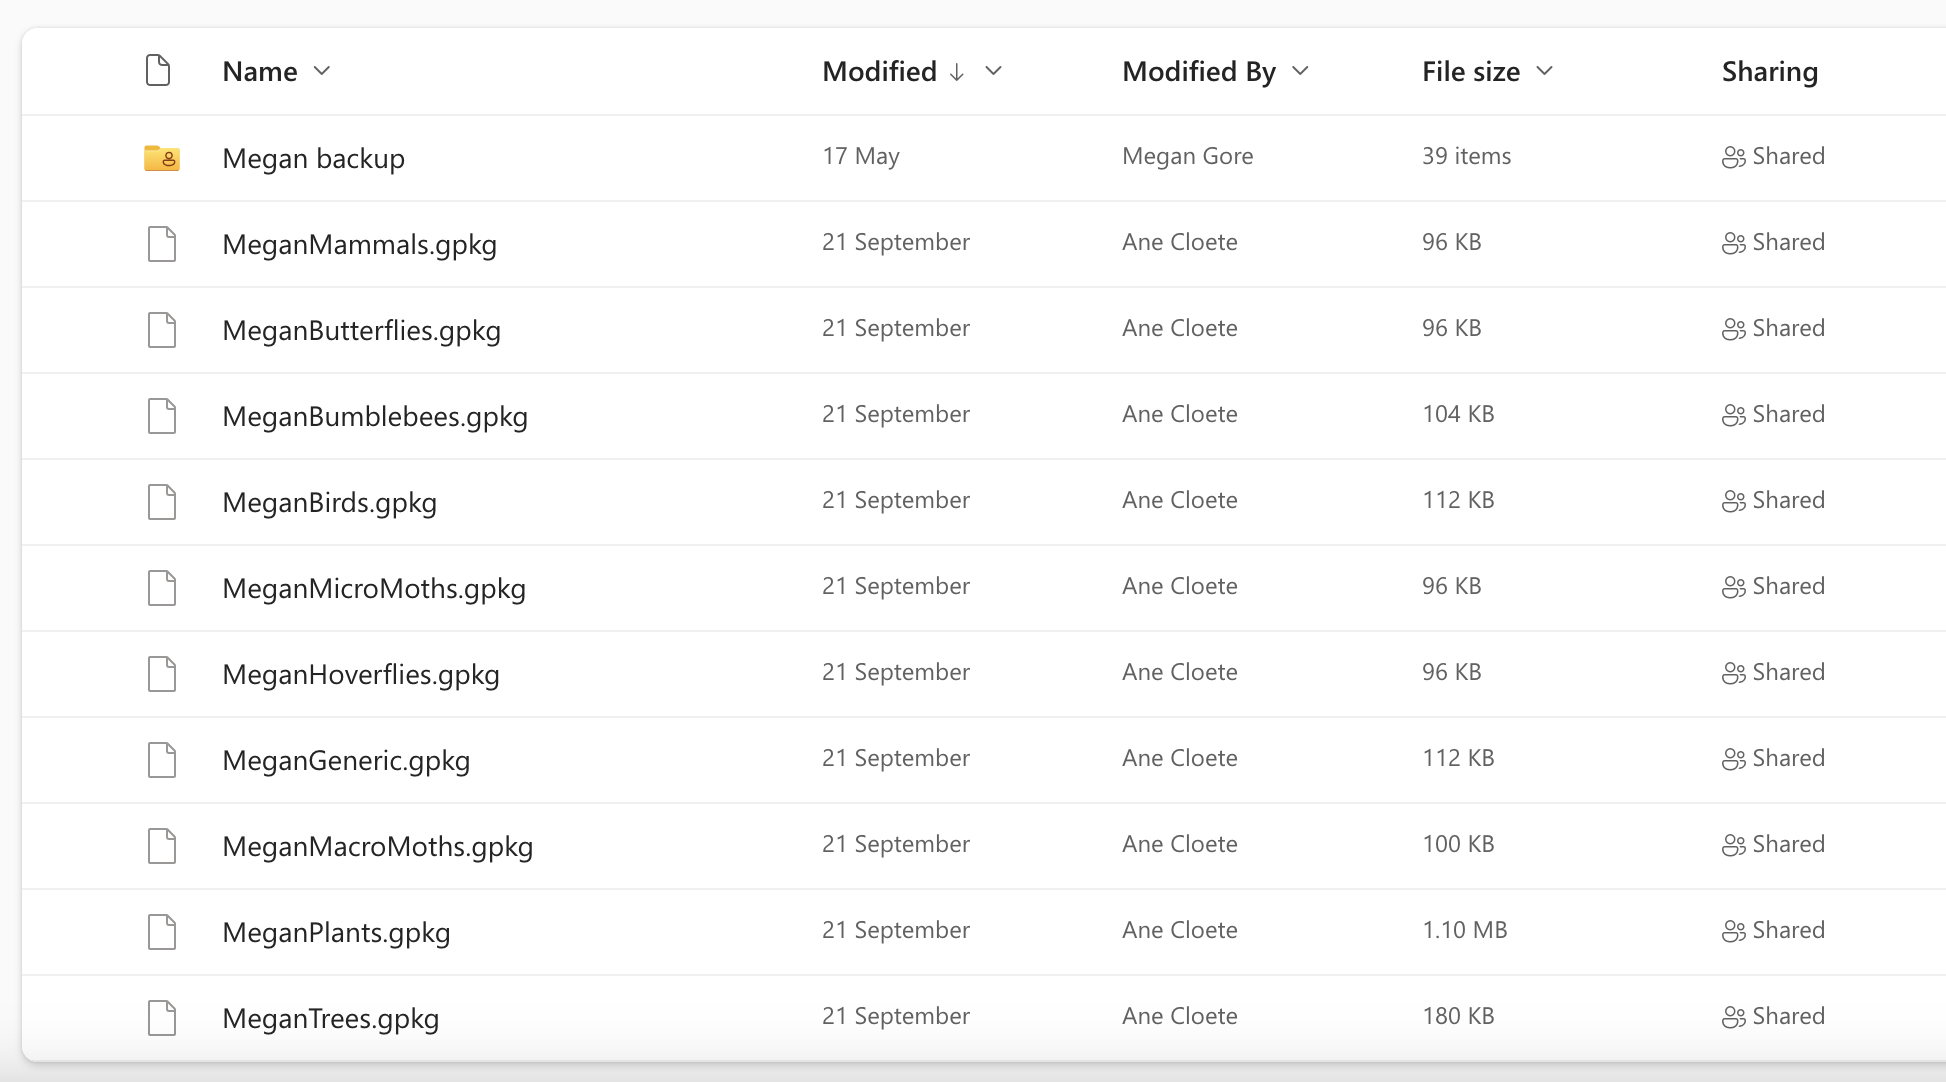
\includegraphics{images/megan_folder.png}

If you don't know what a \href{https://www.geopackage.org/}{geopackage} is, here's a quick description:

A GeoPackage is like a supercharged file for maps and location data. It's a clever way to bundle up all sorts of info---like where things are on a map, pictures, and details about those things. Think of it as a digital suitcase for geography. What makes it cool is that it works on different devices and software without any fuss.

\hypertarget{team_data}{%
\subsection{Team\_Data}\label{team_data}}

This folder contains photos of each student and a word document containing their ``About Me'' descriptions used in the dashboard. The nomenclature and file type is important here. The photo mus''t be saved with their name as the file name and they should be jpg's! Then the word document should be called ``student\_aboutme'' - you can change it if you want, but then you have to change it in the dashboard code as well. Within the document the student descriptions are paragraphs and within the first sentence the student introduces themselves with their names - this is NB. The code will will separate the text into paragraphs and then filter for the student by searching for their name. It's your job to tell everyone to stick to this format and style!

\hypertarget{survey_photos}{%
\subsection{Survey\_Photos}\label{survey_photos}}

All the photos taken while surveying are uploaded here with their unique photo ID as file name. The file name isn't super important for the dashboard as long as it's consisted between their records and the uploaded data. Ensure that all the photos are in the same format (i.e.~jpg) - if not then there is a way to convert them all in one go which I'll mention later.

\hypertarget{bmpdashboard}{%
\section{BMPDashboard}\label{bmpdashboard}}

Here is what you should see:

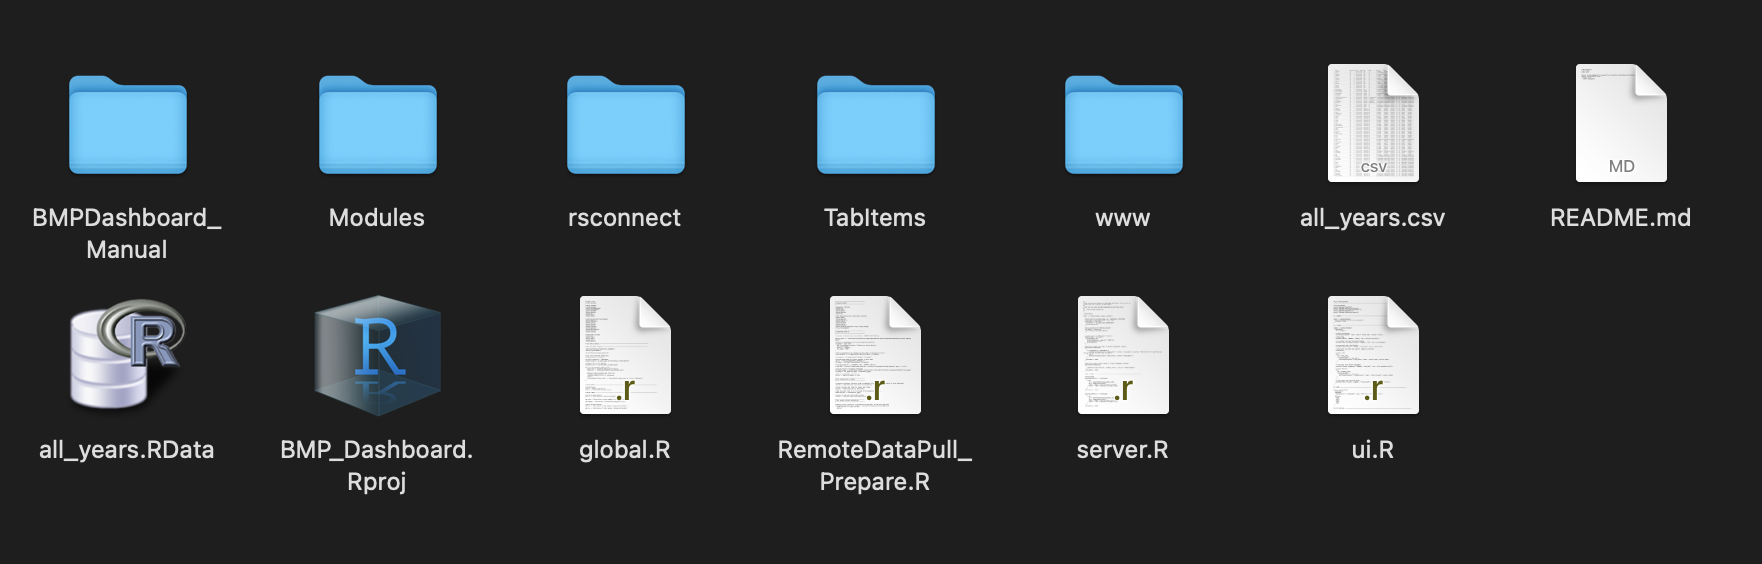
\includegraphics{images/BMPDashboard.png}

\begin{itemize}
\item
  BMPDashboard\_Manual folder
\item
  BMP\_Dashboard.Rproj
\item
  RemoteDataPullPrepare.R
\item
  global.R
\item
  server.R
\item
  ui.R
\item
  Modules folder
\item
  rsconnect folder (you'll only see this once you've published the app to shinyapps.io)
\item
  TabItems folder
\item
  www folder
\item
  README.md
\item
  packages.R
\end{itemize}

If you're familiar with R projects and shiny apps then this should look familiar barring the obvious extras such the as the first folder (which contains the code for this bookdown). Let's quickly go over the rest.

\hypertarget{remotedatapullprepare.r}{%
\subsection{RemoteDataPullPrepare.R}\label{remotedatapullprepare.r}}

This contains the code for pulling the data from OneDrive and preparing it.

\hypertarget{global.r-ui.r-and-server.r}{%
\subsection{global.R, ui.R and server.R}\label{global.r-ui.r-and-server.r}}

These are the main shiny app files!

\hypertarget{tabitems}{%
\subsection{TabItems}\label{tabitems}}

Contains the ui code for each tab in the dashboard (Tab\_About.R, Tab\_KPI.R, Tab\_Record\_Finder.R, Tab\_Student\_Engagement.R and Tab\_Taxa\_Explorer.R). I've done this mostly to keep the ui file clean and comprehensible, but it's slightly annoying for work flow as when you make a change here, you have close the app and then run it again. You could put all the code into the ui script and then if you make changes you only have to reload the app. Up to you!

\hypertarget{modules}{%
\subsection{Modules}\label{modules}}

Contains the code for a custom valuebox which is used throughout the dashboard which I've turned into a shiny module. A Shiny module is like a neat toolkit for creating specific interactive parts of your app without making a mess of your code. It's like having a mini-app inside your bigger app. So, let's say you want a snazzy chart or a dynamic table---you can build that as a Shiny module. It keeps things organized and clean, making your web development life easier. It's like having building blocks for your website, and each block (or module) does a special job, making your site more interactive and user-friendly.

At the moment I've only converted the valuebox into a module, but there are other things that can be turned into modules too! Like the datatables or the bar graphs. Feel free to play around with this!

\hypertarget{www}{%
\subsection{www}\label{www}}

The \textbf{www} folder is like the storage room of your shiny app where you keep all the stuff that makes the outside look awesome. In the \textbf{www} folder, you put things like images, stylesheets (which control how things look), and JavaScript files (for extra functionality). In our \textbf{www} folder you'll find:

\begin{itemize}
\item
  all the survey photos
\item
  a custom css stylesheet (custom.css)
\item
  a copy of the Team\_Data folder with additional objects: doc\_parts.RData and student\_text\_sep.RData
\item
  the allyears.RData object (this is the cleaned dataset which the dashboard uses)
\end{itemize}

\hypertarget{readme.md}{%
\subsection{README.md}\label{readme.md}}

This a plain text file usually written in a simple format called Markdown that contains the description you see on github.

\hypertarget{packages.r}{%
\subsection{packages.R}\label{packages.r}}

This r script contains all code to install and load all the packages required for the dashboard.

\hypertarget{the-data}{%
\chapter{The Data}\label{the-data}}

\hypertarget{setting-up-onedrive}{%
\section{Setting up OneDrive}\label{setting-up-onedrive}}

The following instructions are for Mac users. If you are using windows, you should have OneDrive already installed on your computer.

\begin{enumerate}
\def\labelenumi{\arabic{enumi}.}
\tightlist
\item
  \textbf{Download OneDrive:}

  \begin{itemize}
  \tightlist
  \item
    Go to the Mac App Store on your laptop.
  \item
    Search for ``OneDrive.''
  \item
    Click on ``Get'' or ``Install'' to download the OneDrive app.
  \end{itemize}
\item
  \textbf{Install OneDrive:}

  \begin{itemize}
  \tightlist
  \item
    Once downloaded, open your Applications folder and locate the OneDrive app.
  \item
    Drag the OneDrive app to your Dock for easier access (optional).
  \end{itemize}
\item
  \textbf{Sign In:}

  \begin{itemize}
  \tightlist
  \item
    Open the OneDrive app.
  \item
    Sign in with your university account.
  \item
    Follow the on-screen prompts to set up OneDrive.
  \end{itemize}
\item
  \textbf{Choose Folders to Sync:}

  \begin{itemize}
  \tightlist
  \item
    Once signed in, you'll have the option to choose which folders from your OneDrive cloud storage you want to sync with your Mac.
  \item
    Select the folders you want or choose to sync everything.
  \end{itemize}
\item
  \textbf{Set OneDrive Preferences:}

  \begin{itemize}
  \tightlist
  \item
    Click on the OneDrive icon in the Mac menu bar at the top of your screen.
  \item
    Click on the three dots (More) and select ``Preferences.''
  \item
    Here, you can adjust settings like:

    \begin{itemize}
    \tightlist
    \item
      Starting OneDrive automatically when you sign in to your Mac.
    \item
      Choosing how files are downloaded or uploaded (e.g., over metered networks).
    \item
      Setting up file on-demand (allows you to see all your files without having them downloaded).
    \end{itemize}
  \end{itemize}
\item
  \textbf{Accessing Your Files:}
\end{enumerate}

\begin{itemize}
\tightlist
\item
  A OneDrive folder will now be present in your Mac's Finder. This folder will sync with your online OneDrive storage. { Any files or folders you add to this folder will be automatically uploaded to the cloud, and any changes you make to files in this folder will be reflected in the cloud version.} Read that again! It important that you know that if you change or delete any files in the OneDrive folder on your laptop it will affect the database online.
\end{itemize}

\begin{enumerate}
\def\labelenumi{\arabic{enumi}.}
\setcounter{enumi}{6}
\tightlist
\item
  \textbf{To Unlink or Sign Out:}

  \begin{itemize}
  \tightlist
  \item
    If you ever wish to unlink your account or sign out, click on the OneDrive icon in the Mac menu bar.
  \item
    Click on the three dots (More) and select ``Preferences.''
  \item
    Go to the ``Account'' tab and select ``Unlink this Mac.''
  \end{itemize}
\end{enumerate}

\hypertarget{getting-the-data}{%
\section{Getting the data}\label{getting-the-data}}

First, navigate to the R script called ``packages'' to check whether you have all the required packages, if you don't the script will also install and load them for you. Done!

Now, open the script ``RemoteDataPull\_Prepare''.

The most important first step here is to modify the object ``path\_to\_master'' with the filepath to where ever you have the OneDrive folder on your device and specifically to the main survey folder ``Biodiversity Survey Master''. If you are using a Mac, navigate to the folder in Finder and then in the bottom panel (see below), right click the folder name and select ``Copy''folder name'' as Pathname''.

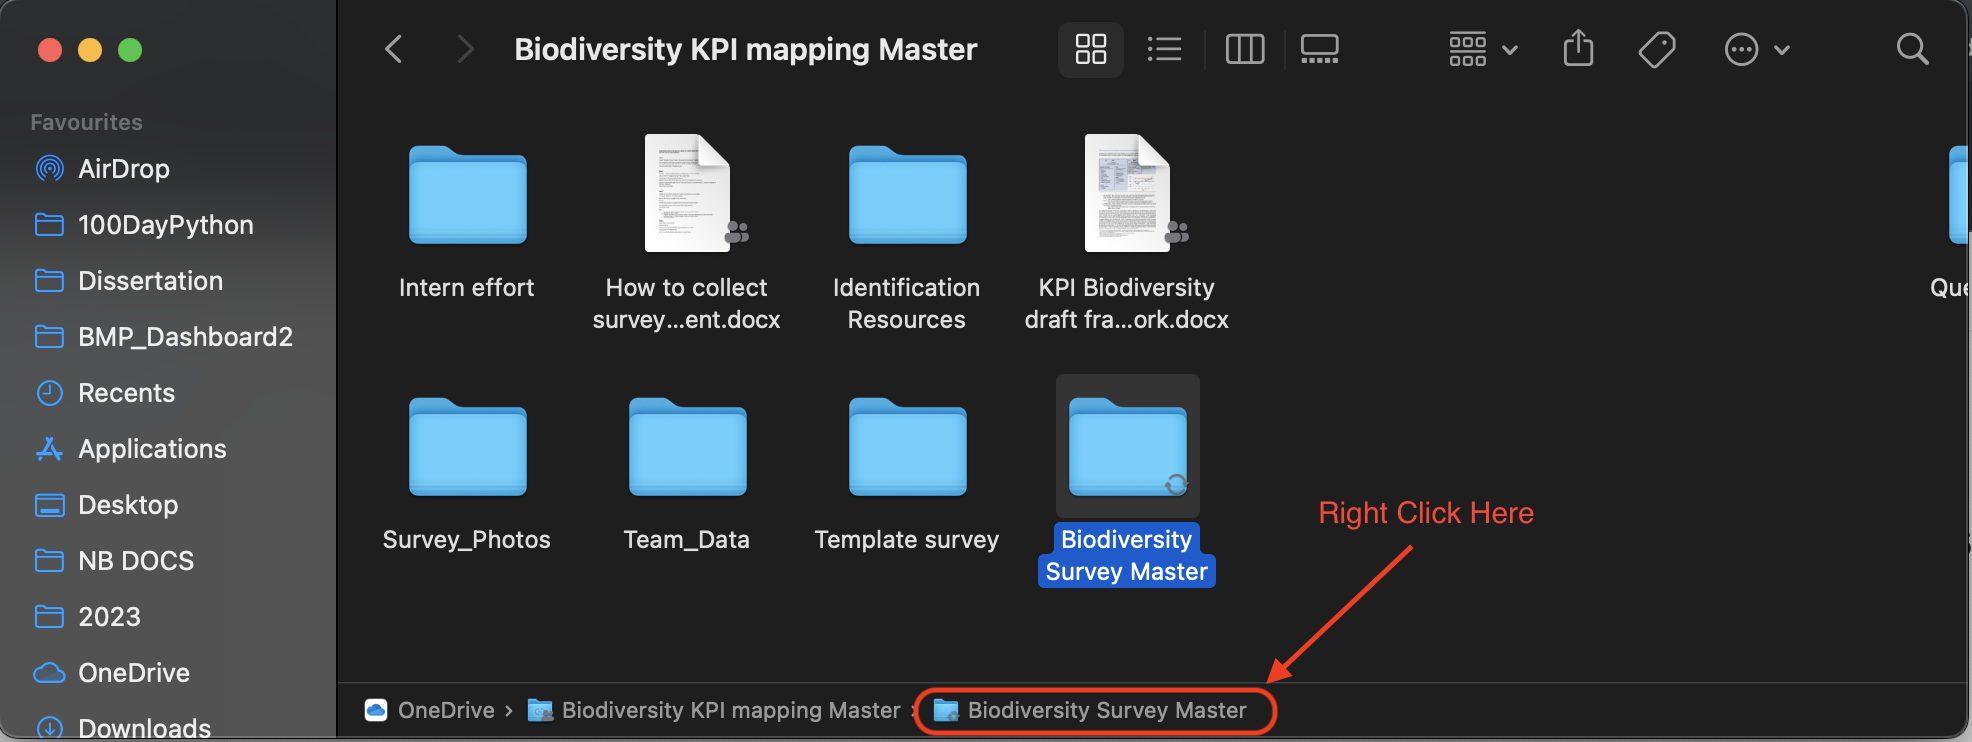
\includegraphics{images/pathname_copy.png}

Let's break down the code:

\begin{enumerate}
\def\labelenumi{\arabic{enumi}.}
\tightlist
\item
  \textbf{Setting the Path to the Master Directory}:
\end{enumerate}

\begin{Shaded}
\begin{Highlighting}[]
\NormalTok{   path\_to\_master }\OtherTok{\textless{}{-}} \StringTok{"/Users/anecloete/Library/CloudStorage/OneDrive{-}UniversityofStAndrews/Biodiversity KPI mapping Master"}
\end{Highlighting}
\end{Shaded}

This line sets a variable called \texttt{path\_to\_master} to the path of the main directory where the geopackage files are located. Paste the pathname you copied here.

\begin{enumerate}
\def\labelenumi{\arabic{enumi}.}
\setcounter{enumi}{1}
\tightlist
\item
  \textbf{Obtaining All Geopackage Files}:
\end{enumerate}

\begin{Shaded}
\begin{Highlighting}[]
\NormalTok{all\_gpkgs }\OtherTok{\textless{}{-}} \FunctionTok{list.files}\NormalTok{(}
  \AttributeTok{path =} \FunctionTok{paste0}\NormalTok{(path\_to\_master,}\StringTok{"/Biodiversity Survey Master"}\NormalTok{),}
  \AttributeTok{recursive =} \ConstantTok{TRUE}\NormalTok{,}
  \AttributeTok{pattern =} \StringTok{"}\SpecialCharTok{\textbackslash{}\textbackslash{}}\StringTok{.gpkg$"}\NormalTok{,}
  \AttributeTok{full.names =} \ConstantTok{TRUE}
\NormalTok{)}
\end{Highlighting}
\end{Shaded}

This code lists all files with the ``.gpkg'' extension in the specified directory and its subdirectories.
- The \texttt{path} argument specifies where to look.
- \texttt{recursive} set to \texttt{TRUE} means it will look in subdirectories as well.
- \texttt{pattern} filters for files ending with ``.gpkg''.
- \texttt{full.names} set to \texttt{TRUE} ensures the full path of each file is returned, not just its name.

\begin{enumerate}
\def\labelenumi{\arabic{enumi}.}
\setcounter{enumi}{2}
\tightlist
\item
  \textbf{Filtering Geopackages with `Habitat\_Polygon' in Their Name}:
\end{enumerate}

\begin{Shaded}
\begin{Highlighting}[]
\NormalTok{   survey\_polygons }\OtherTok{\textless{}{-}}\NormalTok{ all\_gpkgs[}\FunctionTok{grepl}\NormalTok{(}\StringTok{"Habitat\_Polygon"}\NormalTok{, all\_gpkgs)]}
\end{Highlighting}
\end{Shaded}

This filters the \texttt{all\_gpkgs} vector for filenames that contain the substring ``Habitat\_Polygon'' and assigns the subset to \texttt{survey\_polygons}.

\begin{enumerate}
\def\labelenumi{\arabic{enumi}.}
\setcounter{enumi}{3}
\tightlist
\item
  \textbf{Excluding Geopackages Based on Certain Keywords}:
\end{enumerate}

\begin{Shaded}
\begin{Highlighting}[]
\NormalTok{   pattern }\OtherTok{\textless{}{-}} \StringTok{"Polygon|DESKTOP|PC|LAPTOP|Wills"}
\NormalTok{   all\_gpkgs }\OtherTok{\textless{}{-}}\NormalTok{ all\_gpkgs[}\SpecialCharTok{!}\FunctionTok{grepl}\NormalTok{(pattern, all\_gpkgs)]}
\end{Highlighting}
\end{Shaded}

Here, a pattern is defined to exclude geopackages with certain keywords in their names. The \texttt{grepl} function checks for matches, and the \texttt{!} operator negates the condition to exclude matches.

\begin{enumerate}
\def\labelenumi{\arabic{enumi}.}
\setcounter{enumi}{4}
\tightlist
\item
  \textbf{Exclude a Specific Problematic Geopackage}:
\end{enumerate}

\begin{Shaded}
\begin{Highlighting}[]
\NormalTok{   problematic\_gpkg }\OtherTok{\textless{}{-}} \FunctionTok{paste0}\NormalTok{(path\_to\_master,}\StringTok{"/Erica/Erica Backup/Ericabutterflies.gpkg"}\NormalTok{)}
\NormalTok{   all\_gpkgs }\OtherTok{\textless{}{-}}\NormalTok{ all\_gpkgs[all\_gpkgs }\SpecialCharTok{!=}\NormalTok{ problematic\_gpkg]}
\end{Highlighting}
\end{Shaded}

This code defines a specific geopackage file path that is ``problematic'' and then removes this file from the \texttt{all\_gpkgs} vector.

\begin{enumerate}
\def\labelenumi{\arabic{enumi}.}
\setcounter{enumi}{5}
\tightlist
\item
  \textbf{Reading All Geopackages into a List}:
\end{enumerate}

\begin{Shaded}
\begin{Highlighting}[]
\NormalTok{myfiles }\OtherTok{\textless{}{-}} \FunctionTok{lapply}\NormalTok{(all\_gpkgs, st\_read)}
\end{Highlighting}
\end{Shaded}

The \texttt{lapply} function is used here to apply the \texttt{st\_read} function to each file path in the \texttt{all\_gpkgs} vector. The result is a list, with each element being the content of a geopackage file stored as an spatial features dataframe. The \texttt{st\_read} function is part of the \texttt{sf} package in R and is used to read spatial data.

In summary, this code:
- Sets a path to a master directory.
- Lists all geopackage files from this directory and its subdirectories.
- Filters and excludes certain geopackages based on keywords or specific filenames.
- Reads the content of each remaining geopackage file into a list.

\hypertarget{data-cleaning-and-preparation}{%
\section{Data cleaning and preparation}\label{data-cleaning-and-preparation}}

Most of this is self explanatory or is a bit tedious to explain. I would recommended investigating and exploring the data before the cleaning and preparation so that some of the lines make more sense. But here are a few notable things:

\begin{itemize}
\tightlist
\item
  Each student have a backup folder embedded in their folder, these geopackages are removed in line 72
\item
  There is separate geopackage for tree data collected, this is included in the dashboard so is cleaned separately and then joined to the rest.
\item
  The Species column contains the name of the species recorded, whether this is the scientific name, the common name or anything else. So all the naming columns are coalesced into one column called Species.
\item
  Line 135 was necessary because for some reason empty entries in the relevant columns were ``\,'' and not NA
\end{itemize}

Some of the code could be a little less sausage making-ish and could be simplified (somethings were added after the fact etc), feel free to make it more efficient!

\textbf{SUMMARY}:

\begin{enumerate}
\def\labelenumi{\arabic{enumi}.}
\tightlist
\item
  \textbf{Coordinate Transformation}:

  \begin{itemize}
  \tightlist
  \item
    Transforms the coordinate reference system of spatial data to standard latitude and longitude (EPSG:4326).
  \end{itemize}
\end{enumerate}

\begin{Shaded}
\begin{Highlighting}[]
\CommentTok{\# Transform coordinate reference system from WGS 84 / Pseudo{-}Mercator to standard lat long (EPSG:4326)}
\NormalTok{taxa\_dat }\OtherTok{\textless{}{-}} \FunctionTok{lapply}\NormalTok{(myfiles, }\ControlFlowTok{function}\NormalTok{(x) }\FunctionTok{st\_transform}\NormalTok{(x, }\DecValTok{4326}\NormalTok{))}
\end{Highlighting}
\end{Shaded}

\begin{enumerate}
\def\labelenumi{\arabic{enumi}.}
\setcounter{enumi}{1}
\tightlist
\item
  \textbf{Data Conversions}:

  \begin{itemize}
  \tightlist
  \item
    Converts the spatial data frames to regular data frames.
  \item
    Names each data frame in the list based on the geopackage filename.
  \item
    Removes duplicate data frames based on their names.
  \end{itemize}
\end{enumerate}

\begin{Shaded}
\begin{Highlighting}[]
\CommentTok{\# Convert spatial data frames to regular data frames}
\NormalTok{taxa\_dat }\OtherTok{\textless{}{-}} \FunctionTok{lapply}\NormalTok{(taxa\_dat, as.data.frame)}

\CommentTok{\# Name each data frame in the list based on the geopackage filename}
\FunctionTok{names}\NormalTok{(taxa\_dat) }\OtherTok{\textless{}{-}} \FunctionTok{basename}\NormalTok{(all\_gpkgs)}

\CommentTok{\# Remove any duplicate data frames by name}
\NormalTok{taxa\_dat }\OtherTok{\textless{}{-}}\NormalTok{ taxa\_dat[}\SpecialCharTok{!}\FunctionTok{duplicated}\NormalTok{(}\FunctionTok{names}\NormalTok{(taxa\_dat))]}
\end{Highlighting}
\end{Shaded}

\begin{enumerate}
\def\labelenumi{\arabic{enumi}.}
\setcounter{enumi}{2}
\tightlist
\item
  \textbf{Tree Entries Package Preparation}:

  \begin{itemize}
  \tightlist
  \item
    Modifies columns for a specific geopackage (`Tree Species Entries.gpkg') to ensure compatibility with subsequent operations.
  \item
    Cleans and modifies species names.
  \item
    Sets certain columns to specific values or \texttt{NA}.
  \item
    Filters and selects specific columns.
  \end{itemize}
\end{enumerate}

\begin{Shaded}
\begin{Highlighting}[]
\CommentTok{\# Modify certain columns for \textquotesingle{}Tree Species Entries.gpkg\textquotesingle{} so that bind\_rows works }
\NormalTok{taxa\_dat}\SpecialCharTok{$}\StringTok{\textasciigrave{}}\AttributeTok{Tree Species Entries.gpkg}\StringTok{\textasciigrave{}} \OtherTok{\textless{}{-}}\NormalTok{ taxa\_dat}\SpecialCharTok{$}\StringTok{\textasciigrave{}}\AttributeTok{Tree Species Entries.gpkg}\StringTok{\textasciigrave{}} \SpecialCharTok{\%\textgreater{}\%}
  \FunctionTok{rename}\NormalTok{(}\AttributeTok{Species =} \DecValTok{1}\NormalTok{, }\AttributeTok{Date =} \DecValTok{2}\NormalTok{) }\SpecialCharTok{\%\textgreater{}\%}
  \FunctionTok{mutate}\NormalTok{(}
    \AttributeTok{Species =} \FunctionTok{case\_when}\NormalTok{(}
\NormalTok{      Species }\SpecialCharTok{\%in\%} \FunctionTok{c}\NormalTok{(}\StringTok{"unknown/other"}\NormalTok{, }\StringTok{"Unknown/other"}\NormalTok{) }\SpecialCharTok{\textasciitilde{}}\NormalTok{ comments.unlisted.species,}
\NormalTok{      Species }\SpecialCharTok{==} \StringTok{"Unknown young pine "} \SpecialCharTok{\textasciitilde{}} \StringTok{"Unknown young pine"}\NormalTok{,}
\NormalTok{      Species }\SpecialCharTok{==} \StringTok{"Willow x10"} \SpecialCharTok{\textasciitilde{}} \StringTok{"Willow"}\NormalTok{,}
      \ConstantTok{TRUE} \SpecialCharTok{\textasciitilde{}}\NormalTok{ Species}
\NormalTok{    ),}
    \AttributeTok{taxa =} \StringTok{"Vascular Plants"}\NormalTok{,}
    \AttributeTok{Observer =} \ConstantTok{NA}\NormalTok{,}
    \AttributeTok{photoid =} \ConstantTok{NA}\NormalTok{,}
    \AttributeTok{Count =} \ConstantTok{NA}\NormalTok{,}
    \AttributeTok{Other =} \ConstantTok{NA}\NormalTok{,}
    \AttributeTok{Speciesful =} \ConstantTok{NA}
\NormalTok{  ) }\SpecialCharTok{\%\textgreater{}\%}
  \FunctionTok{filter}\NormalTok{(Species }\SpecialCharTok{!=} \StringTok{""}\NormalTok{) }\SpecialCharTok{\%\textgreater{}\%}
  \FunctionTok{select}\NormalTok{(Species, Date, taxa, Count)}
\end{Highlighting}
\end{Shaded}

\begin{enumerate}
\def\labelenumi{\arabic{enumi}.}
\setcounter{enumi}{3}
\tightlist
\item
  \textbf{Date Processing}:

  \begin{itemize}
  \tightlist
  \item
    Converts, splits, and extracts components (year, month, day) of the `Date' column.
  \end{itemize}
\end{enumerate}

\begin{Shaded}
\begin{Highlighting}[]
\CommentTok{\# Date Processing: Convert, split and extract components of the \textquotesingle{}Date\textquotesingle{} column}
\NormalTok{taxa\_dat }\OtherTok{\textless{}{-}} \FunctionTok{lapply}\NormalTok{(taxa\_dat, }\ControlFlowTok{function}\NormalTok{(df) \{}
  
\NormalTok{  df}\SpecialCharTok{$}\NormalTok{Date }\OtherTok{\textless{}{-}} \FunctionTok{as.character}\NormalTok{(df}\SpecialCharTok{$}\NormalTok{Date)}
  
\NormalTok{  df }\OtherTok{\textless{}{-}}\NormalTok{ df }\SpecialCharTok{\%\textgreater{}\%}
    \FunctionTok{separate}\NormalTok{(Date, }\AttributeTok{into =} \FunctionTok{c}\NormalTok{(}\StringTok{"date"}\NormalTok{, }\StringTok{"time"}\NormalTok{), }\AttributeTok{sep =} \StringTok{" (?=[\^{} ]+$)"}\NormalTok{) }\SpecialCharTok{\%\textgreater{}\%}
    \FunctionTok{mutate}\NormalTok{(}
      \AttributeTok{date =} \FunctionTok{ymd}\NormalTok{(}\FunctionTok{gsub}\NormalTok{(}\StringTok{"/"}\NormalTok{, }\StringTok{"{-}"}\NormalTok{, date)),}
      \AttributeTok{year =} \FunctionTok{year}\NormalTok{(date),}
      \AttributeTok{month =} \FunctionTok{month}\NormalTok{(date),}
      \AttributeTok{day =} \FunctionTok{day}\NormalTok{(date)}
\NormalTok{    )}
  \FunctionTok{return}\NormalTok{(df)}
\NormalTok{\})}
\end{Highlighting}
\end{Shaded}

\begin{enumerate}
\def\labelenumi{\arabic{enumi}.}
\setcounter{enumi}{4}
\tightlist
\item
  \textbf{Tree Data Extraction}:

  \begin{itemize}
  \tightlist
  \item
    Removes the tree data frame from the list and stores it separately.
  \end{itemize}
\end{enumerate}

\begin{Shaded}
\begin{Highlighting}[]
\CommentTok{\# Extract and remove the tree dataframe from the list}
\NormalTok{tree\_data }\OtherTok{\textless{}{-}}\NormalTok{ taxa\_dat}\SpecialCharTok{$}\StringTok{\textasciigrave{}}\AttributeTok{Tree Species Entries.gpkg}\StringTok{\textasciigrave{}}
\NormalTok{taxa\_dat}\SpecialCharTok{$}\StringTok{\textasciigrave{}}\AttributeTok{Tree Species Entries.gpkg}\StringTok{\textasciigrave{}} \OtherTok{\textless{}{-}} \ConstantTok{NULL}
\end{Highlighting}
\end{Shaded}

\begin{enumerate}
\def\labelenumi{\arabic{enumi}.}
\setcounter{enumi}{5}
\tightlist
\item
  \textbf{Combining Data}:

  \begin{itemize}
  \tightlist
  \item
    Merges all data frames in the list into a single data frame.
  \end{itemize}
\end{enumerate}

\begin{Shaded}
\begin{Highlighting}[]
\CommentTok{\# Combine all data frames in the list into a single data frame}
\NormalTok{taxa\_comb }\OtherTok{\textless{}{-}} \FunctionTok{bind\_rows}\NormalTok{(taxa\_dat)}
\end{Highlighting}
\end{Shaded}

\begin{enumerate}
\def\labelenumi{\arabic{enumi}.}
\setcounter{enumi}{6}
\tightlist
\item
  \textbf{Data Cleaning and Transformation}:

  \begin{itemize}
  \tightlist
  \item
    Performs several operations to clean and transform the combined data, including:

    \begin{itemize}
    \tightlist
    \item
      Date conversions and modifications.
    \item
      Handling missing values.
    \item
      Excluding certain records.
    \item
      Recoding values in various columns.
    \item
      Selecting and renaming columns.
    \end{itemize}
  \end{itemize}
\end{enumerate}

\begin{Shaded}
\begin{Highlighting}[]
\CommentTok{\# Clean and transform taxa data for further analysis}
\NormalTok{taxa\_clean }\OtherTok{\textless{}{-}}\NormalTok{ taxa\_comb }\SpecialCharTok{\%\textgreater{}\%}
  \FunctionTok{drop\_na}\NormalTok{(taxa) }\SpecialCharTok{\%\textgreater{}\%}
  \FunctionTok{as.character}\NormalTok{(df}\SpecialCharTok{$}\NormalTok{Date) }\SpecialCharTok{\%\textgreater{}\%} 
  \FunctionTok{separate}\NormalTok{(Date, }\AttributeTok{into =} \FunctionTok{c}\NormalTok{(}\StringTok{"date"}\NormalTok{, }\StringTok{"time"}\NormalTok{), }\AttributeTok{sep =} \StringTok{" (?=[\^{} ]+$)"}\NormalTok{) }\SpecialCharTok{\%\textgreater{}\%}
  \FunctionTok{mutate}\NormalTok{(}
    \AttributeTok{date =} \FunctionTok{ymd}\NormalTok{(}\FunctionTok{gsub}\NormalTok{(}\StringTok{"/"}\NormalTok{, }\StringTok{"{-}"}\NormalTok{, date)),}
    \AttributeTok{year =} \FunctionTok{year}\NormalTok{(date),}
    \AttributeTok{month =} \FunctionTok{month}\NormalTok{(date),}
    \AttributeTok{day =} \FunctionTok{day}\NormalTok{(date)}
\NormalTok{  ) }\SpecialCharTok{\%\textgreater{}\%} 
  \FunctionTok{filter}\NormalTok{(}\SpecialCharTok{!}\NormalTok{(taxa }\SpecialCharTok{==} \StringTok{"hoverfly"} \SpecialCharTok{\&}\NormalTok{ Observer }\SpecialCharTok{==} \StringTok{"Erica"}\NormalTok{)) }\SpecialCharTok{\%\textgreater{}\%} \CommentTok{\# remove Erica hoverfly entries }
  \FunctionTok{unite}\NormalTok{(collapsed\_species, specieslatin}\SpecialCharTok{:}\NormalTok{seaweedlatin, }\AttributeTok{sep =} \StringTok{","}\NormalTok{, }\AttributeTok{na.rm =} \ConstantTok{TRUE}\NormalTok{) }\SpecialCharTok{\%\textgreater{}\%}
  \FunctionTok{mutate\_at}\NormalTok{(}\FunctionTok{vars}\NormalTok{(Species, collapsed\_species), na\_if, }\StringTok{""}\NormalTok{) }\SpecialCharTok{\%\textgreater{}\%}
  \FunctionTok{mutate}\NormalTok{(}
    \AttributeTok{Species =} \FunctionTok{coalesce}\NormalTok{(Species, SpeciesSci, Speciesfull, collapsed\_species, species, Other),}
    \AttributeTok{photoid =} \FunctionTok{if\_else}\NormalTok{(}\FunctionTok{is.na}\NormalTok{(photoid), }\ConstantTok{NA}\NormalTok{, }\FunctionTok{paste0}\NormalTok{(photoid, }\StringTok{".jpg"}\NormalTok{)),}
    \AttributeTok{Count =} \FunctionTok{ifelse}\NormalTok{(}\FunctionTok{is.na}\NormalTok{(Count), }\DecValTok{1}\NormalTok{, Count),}
    \AttributeTok{taxa =} \FunctionTok{recode}\NormalTok{(taxa, }\AttributeTok{tree =} \StringTok{"Vascular Plants"}\NormalTok{),}
    \AttributeTok{year =} \FunctionTok{recode}\NormalTok{(year, }\StringTok{\textasciigrave{}}\AttributeTok{2023}\StringTok{\textasciigrave{}} \OtherTok{=} \StringTok{"2022/2023"}\NormalTok{, }\StringTok{\textasciigrave{}}\AttributeTok{2022}\StringTok{\textasciigrave{}} \OtherTok{=} \StringTok{"2022/2023"}\NormalTok{)}
\NormalTok{  ) }\SpecialCharTok{\%\textgreater{}\%}
  \FunctionTok{filter}\NormalTok{(}\SpecialCharTok{!}\FunctionTok{str\_detect}\NormalTok{(Species, }\StringTok{"(?i)unknown"}\NormalTok{), taxa }\SpecialCharTok{!=} \StringTok{"bee"}\NormalTok{) }\SpecialCharTok{\%\textgreater{}\%}
  \FunctionTok{filter\_at}\NormalTok{(}\FunctionTok{vars}\NormalTok{(taxa, Observer), }\FunctionTok{all\_vars}\NormalTok{(}\SpecialCharTok{!}\FunctionTok{is.na}\NormalTok{(.))) }\SpecialCharTok{\%\textgreater{}\%}
  \FunctionTok{mutate}\NormalTok{(}
    \AttributeTok{taxa =} \FunctionTok{recode}\NormalTok{(taxa, }
                  \AttributeTok{plant =} \StringTok{"Vascular Plants"}\NormalTok{,}
                  \AttributeTok{bird =} \StringTok{"Birds"}\NormalTok{,}
                  \AttributeTok{macromoth =} \StringTok{"Macromoths"}\NormalTok{,}
                  \AttributeTok{micromoth =} \StringTok{"Micromoths"}\NormalTok{,}
                  \AttributeTok{butterfly =} \StringTok{"Butterflies"}\NormalTok{,}
                  \AttributeTok{dragonfly =} \StringTok{"Dragonflies"}\NormalTok{,}
                  \AttributeTok{hoverfly =} \StringTok{"Hoverflies"}\NormalTok{,}
                  \AttributeTok{bat =} \StringTok{"Bats"}\NormalTok{,}
                  \AttributeTok{amphibian =} \StringTok{"Amphibians"}\NormalTok{,}
                  \AttributeTok{reptileamphibian =} \StringTok{"Amphibians"}\NormalTok{,}
                  \AttributeTok{bumblebee =} \StringTok{"Bumblebee"}\NormalTok{,}
                  \AttributeTok{mammal =} \StringTok{"Mammals"}\NormalTok{,}
                  \AttributeTok{ladybird =} \StringTok{"Ladybirds"}\NormalTok{,}
                  \AttributeTok{tree =} \StringTok{"Vascular Plants"}\NormalTok{),}
    \AttributeTok{year =} \FunctionTok{recode}\NormalTok{(year,}
                  \StringTok{"2023"} \OtherTok{=} \StringTok{"2022/2023"}\NormalTok{,}
                  \StringTok{"2022"} \OtherTok{=} \StringTok{"2022/2023"}\NormalTok{),}
    \AttributeTok{Observer =} \FunctionTok{recode}\NormalTok{(Observer,}
                      \AttributeTok{Other1 =} \StringTok{"Cori"}\NormalTok{)) }\SpecialCharTok{\%\textgreater{}\%}
  \FunctionTok{select}\NormalTok{(Species, SpeciesSci, Count, date, Observer, taxa, photoid, geometry, year, day) }\SpecialCharTok{\%\textgreater{}\%}
  \FunctionTok{rename}\NormalTok{(}
    \AttributeTok{Date =}\NormalTok{ date,}
    \AttributeTok{Taxa =}\NormalTok{ taxa,}
    \AttributeTok{PhotoID =}\NormalTok{ photoid}
\NormalTok{  )}
\end{Highlighting}
\end{Shaded}

\begin{enumerate}
\def\labelenumi{\arabic{enumi}.}
\setcounter{enumi}{7}
\tightlist
\item
  \textbf{Merging Tree Data with Cleaned Data}:

  \begin{itemize}
  \tightlist
  \item
    Prepares the tree data to be merged with the cleaned data.
  \item
    Merges both datasets.
  \end{itemize}
\end{enumerate}

\begin{Shaded}
\begin{Highlighting}[]
\CommentTok{\# tree data prep for bind}
\NormalTok{tree\_data }\OtherTok{\textless{}{-}}\NormalTok{ tree\_data }\SpecialCharTok{\%\textgreater{}\%}
  \FunctionTok{mutate}\NormalTok{(}
    \AttributeTok{year =} \FunctionTok{ifelse}\NormalTok{(year }\SpecialCharTok{==} \StringTok{"2023"} \SpecialCharTok{|}\NormalTok{ year }\SpecialCharTok{==} \StringTok{"2022"}\NormalTok{, }\StringTok{"2022/2023"}\NormalTok{, year),}
    \AttributeTok{Count =} \DecValTok{1} \CommentTok{\# add column count }
\NormalTok{  ) }\SpecialCharTok{\%\textgreater{}\%}
  \FunctionTok{rename}\NormalTok{(}
    \AttributeTok{Date =}\NormalTok{ date,}
    \AttributeTok{Taxa =}\NormalTok{ taxa}
\NormalTok{  )}

\CommentTok{\# Merge tree data with the cleaned data}
\NormalTok{all\_years }\OtherTok{\textless{}{-}} \FunctionTok{bind\_rows}\NormalTok{(taxa\_clean, tree\_data)}
\end{Highlighting}
\end{Shaded}

\begin{enumerate}
\def\labelenumi{\arabic{enumi}.}
\setcounter{enumi}{8}
\tightlist
\item
  \textbf{Geometry Processing}:

  \begin{itemize}
  \tightlist
  \item
    Splits the geometry column into separate latitude and longitude columns.
  \end{itemize}
\end{enumerate}

\begin{Shaded}
\begin{Highlighting}[]
\CommentTok{\# split into lat and long for mapping }
\NormalTok{all\_years }\OtherTok{\textless{}{-}}\NormalTok{ all\_years }\SpecialCharTok{\%\textgreater{}\%} \FunctionTok{mutate}\NormalTok{(}\AttributeTok{long =} \FunctionTok{unlist}\NormalTok{(}\FunctionTok{map}\NormalTok{(geometry,}\DecValTok{1}\NormalTok{)),}
           \AttributeTok{lat =} \FunctionTok{unlist}\NormalTok{(}\FunctionTok{map}\NormalTok{(geometry,}\DecValTok{2}\NormalTok{)))}
\end{Highlighting}
\end{Shaded}

\begin{enumerate}
\def\labelenumi{\arabic{enumi}.}
\setcounter{enumi}{9}
\tightlist
\item
  \textbf{Saving the Resulting Data}:

  \begin{itemize}
  \tightlist
  \item
    Saves the final data frame both as an RData object and as a CSV file.
  \end{itemize}
\end{enumerate}

\begin{Shaded}
\begin{Highlighting}[]
\CommentTok{\# Save the resulting dataframe}
\FunctionTok{save}\NormalTok{(all\_years, }\AttributeTok{file =} \StringTok{"all\_years.RData"}\NormalTok{)}
\FunctionTok{write.csv}\NormalTok{(all\_years, }\AttributeTok{file =} \StringTok{"all\_years.csv"}\NormalTok{)}
\end{Highlighting}
\end{Shaded}

\hypertarget{pulling-photos-and-documents-from-onedrive}{%
\section{Pulling photos and documents from OneDrive}\label{pulling-photos-and-documents-from-onedrive}}

\hypertarget{photos}{%
\subsection{Photos}\label{photos}}

\begin{enumerate}
\def\labelenumi{\arabic{enumi}.}
\tightlist
\item
  \textbf{Reading Team Photos from a Directory}:
\end{enumerate}

\begin{Shaded}
\begin{Highlighting}[]
   \CommentTok{\# read in all photo files within Survey\_Photos in OneDrive Folder}
\NormalTok{   all\_Tphotos }\OtherTok{\textless{}{-}} \FunctionTok{list.files}\NormalTok{(}
     \AttributeTok{path =}   \FunctionTok{paste0}\NormalTok{(path\_to\_master,}\StringTok{"/Team\_data"}\NormalTok{),}
     \AttributeTok{recursive =} \ConstantTok{TRUE}\NormalTok{,}
     \AttributeTok{pattern =} \StringTok{"}\SpecialCharTok{\textbackslash{}\textbackslash{}}\StringTok{.jpg$"}\NormalTok{,}
     \AttributeTok{full.names =} \ConstantTok{FALSE}
\NormalTok{   )}
\end{Highlighting}
\end{Shaded}

This is the same as the first few lines of code, except that the path is constructed by appending ``/Team\_data'' to the \texttt{path\_to\_master}.

The result is stored in \texttt{all\_Tphotos}, which will be a vector of filenames (with ``.jpg'' extension) from the specified directory and its subdirectories.

\begin{enumerate}
\def\labelenumi{\arabic{enumi}.}
\setcounter{enumi}{1}
\tightlist
\item
  \textbf{Constructing a Destination Path for Team Photos}:
\end{enumerate}

\begin{Shaded}
\begin{Highlighting}[]
\NormalTok{   www\_Tfolder\_path }\OtherTok{\textless{}{-}} \FunctionTok{file.path}\NormalTok{(}\FunctionTok{getwd}\NormalTok{(), }\StringTok{"www/Team\_Data"}\NormalTok{)}
\end{Highlighting}
\end{Shaded}

This line constructs a path by combining the current working directory (obtained using \texttt{getwd()}) with ``www/Team\_Data''.

\begin{enumerate}
\def\labelenumi{\arabic{enumi}.}
\setcounter{enumi}{2}
\tightlist
\item
  \textbf{Copying the Team Photos}:
\end{enumerate}

\begin{Shaded}
\begin{Highlighting}[]
\NormalTok{   photo\_move }\OtherTok{\textless{}{-}} \FunctionTok{file.copy}\NormalTok{(}
     \AttributeTok{from =} \FunctionTok{file.path}\NormalTok{(}\FunctionTok{paste0}\NormalTok{(path\_to\_master,}\StringTok{"/Team\_data"}\NormalTok{), all\_Tphotos),}
     \AttributeTok{to =} \FunctionTok{file.path}\NormalTok{(}\FunctionTok{paste}\NormalTok{(www\_Tfolder\_path), all\_Tphotos)}
\NormalTok{   )}
\end{Highlighting}
\end{Shaded}

Here, \texttt{file.copy} is used to copy files. The \texttt{from} argument constructs the full paths of the source files, and the \texttt{to} argument constructs the full paths of the destination. The photos are copied from the source directory to the destination.

The same process as above is then done for the Survey Photos.

In summary, the code is designed to:

\begin{itemize}
\tightlist
\item
  Read all ``.jpg'' files from ``Team\_data'' and ``Survey\_Photos'' directories (including subdirectories).
\item
  Copy those files to two new destinations under the ``www'' folder in the current working directory.
\end{itemize}

\hypertarget{documents}{%
\subsection{Documents}\label{documents}}

The code for downloading and saving the students' about me descriptions is very similar to the process above. The only addition is that the text of the ``student\_aboutme'' word document is then extracted and saved into an object called ``student\_text''. Then the text is split into paragraphs.

\hypertarget{things-to-think-about}{%
\section{Things to think about}\label{things-to-think-about}}

How will the next years data be included? In the same folder? New QGIS folder?

\hypertarget{footnotes-and-citations}{%
\chapter{Footnotes and citations}\label{footnotes-and-citations}}

\hypertarget{footnotes}{%
\section{Footnotes}\label{footnotes}}

Footnotes are put inside the square brackets after a caret \texttt{\^{}{[}{]}}. Like this one \footnote{This is a footnote.}.

\hypertarget{citations}{%
\section{Citations}\label{citations}}

Reference items in your bibliography file(s) using \texttt{@key}.

For example, we are using the \textbf{bookdown} package \citep{R-bookdown} (check out the last code chunk in index.Rmd to see how this citation key was added) in this sample book, which was built on top of R Markdown and \textbf{knitr} \citep{xie2015} (this citation was added manually in an external file book.bib).
Note that the \texttt{.bib} files need to be listed in the index.Rmd with the YAML \texttt{bibliography} key.

The RStudio Visual Markdown Editor can also make it easier to insert citations: \url{https://rstudio.github.io/visual-markdown-editing/\#/citations}

\hypertarget{blocks}{%
\chapter{Blocks}\label{blocks}}

\hypertarget{equations}{%
\section{Equations}\label{equations}}

Here is an equation.

\begin{equation} 
  f\left(k\right) = \binom{n}{k} p^k\left(1-p\right)^{n-k}
  \label{eq:binom}
\end{equation}

You may refer to using \texttt{\textbackslash{}@ref(eq:binom)}, like see Equation \eqref{eq:binom}.

\hypertarget{theorems-and-proofs}{%
\section{Theorems and proofs}\label{theorems-and-proofs}}

Labeled theorems can be referenced in text using \texttt{\textbackslash{}@ref(thm:tri)}, for example, check out this smart theorem \ref{thm:tri}.

\begin{theorem}
\protect\hypertarget{thm:tri}{}\label{thm:tri}For a right triangle, if \(c\) denotes the \emph{length} of the hypotenuse
and \(a\) and \(b\) denote the lengths of the \textbf{other} two sides, we have
\[a^2 + b^2 = c^2\]
\end{theorem}

Read more here \url{https://bookdown.org/yihui/bookdown/markdown-extensions-by-bookdown.html}.

\hypertarget{callout-blocks}{%
\section{Callout blocks}\label{callout-blocks}}

The R Markdown Cookbook provides more help on how to use custom blocks to design your own callouts: \url{https://bookdown.org/yihui/rmarkdown-cookbook/custom-blocks.html}

\hypertarget{next-steps}{%
\chapter{Next Steps}\label{next-steps}}

Here is a list of things that need to be done:

\hypertarget{different-years-different-data}{%
\section{Different years different data:}\label{different-years-different-data}}

Currently, the dashboard works a dataset containing data for multiple years - I created a fake dataset for the next academic year as a subset of the 2023 data. The data is combined into the all\_years.RData. It might be better to have separate datasets and store them in a list, its up to you. The next point will influence this too.

\hypertarget{data-download-and-clean-automation}{%
\section{Data download and clean automation:}\label{data-download-and-clean-automation}}

The pulling and preparing of the data should be made automatic, i.e.~everyday during the survey season the data should be pulled from OneDrive, cleaned and uploaded to the dashboard. However, as more data is collected it will probably be better to upload the data to OneDrive (i.e.~not host it on your laptop or shiny server) and have the dashboard pull the data from OneDrive. This will also affect how the dashboard accesses separate years data.

\hypertarget{survey-photos}{%
\section{Survey Photos:}\label{survey-photos}}

The same also applies to the photos. It might be better to pull the photos directly from OneDrive in the app. I'm not sure how to do this and maybe there's a different way to store and retrieve the photos.

  \bibliography{book.bib,packages.bib}

\end{document}
